% Figure from MATH 556 notes, section 11. Compile with the notes preamble.
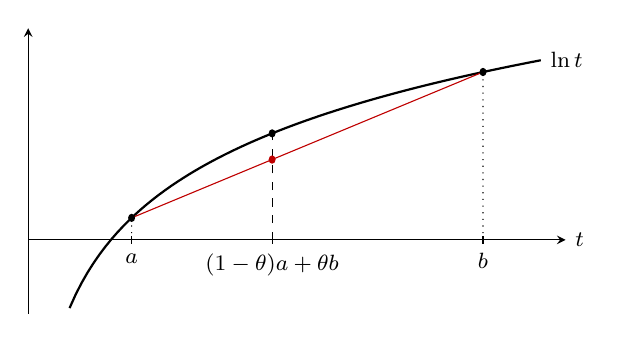
\begin{tikzpicture}[xscale=1.05, yscale=1.25, >=stealth]
    \draw[->] (0,-0.75) -- (0,2.15);
    \draw[->] (0,0) -- (6.5,0) node[right, font=\footnotesize] {$t$};
    \draw[thick, domain=0.5:6.2, samples=80] plot (\x, {ln(\x)});
    \node[right, font=\footnotesize] at (6.2,{ln(6.2)}) {$\ln t$};
    \pgfmathsetmacro{\a}{1.25}
    \pgfmathsetmacro{\b}{5.5}
    \pgfmathsetmacro{\m}{0.6*\a+0.4*\b}
    \coordinate (A) at (\a,{ln(\a)});
    \coordinate (B) at (\b,{ln(\b)});
    \draw[red!75!black] (A) -- (B);
    \draw[dotted] (\a,0) -- (A);
    \draw[dotted] (\b,0) -- (B);
    \draw[dashed] (\m,0) -- (\m,{ln(\m)});
    \fill (A) circle (1.2pt);
    \fill (B) circle (1.2pt);
    \fill (\m,{ln(\m)}) circle (1.2pt);
    \fill[red!75!black] (\m,{0.6*ln(\a)+0.4*ln(\b)}) circle (1.2pt);
    \foreach \x in {\a,\b,\m} \draw (\x,0.04) -- (\x,-0.04);
    \node[below, font=\footnotesize] at (\a,-0.04) {$a$};
    \node[below, font=\footnotesize] at (\b,-0.04) {$b$};
    \node[below, font=\footnotesize] at (\m,-0.04) {$(1-\theta)a + \theta b$};
\end{tikzpicture}
